\documentclass[sigconf, 10pt]{acmart}
\usepackage{tikz}
\usepackage{pgfplots}
\pgfplotsset{compat=1.18}
\usepackage{url}
\usepackage{listings}
\usetikzlibrary{arrows.meta, positioning, shapes.geometric}
\lstset{basicstyle=\small\ttfamily,columns=fullflexible}
\title{T81: A Ternary-Native Stack for Deterministic ML Execution via Metadata Propagation}
\author{t81dev}
\affiliation{%
\institution{The T81 Foundation}
\city{}
\state{}
\country{}
}
\renewcommand{\shortauthors}{The T81 Foundation Collective}
\begin{document}
\begin{abstract}
Modern computing stacks, particularly those for machine learning and systems programming, suffer from pervasive non-determinism. Seemingly identical builds can produce different artifacts, toolchains can exhibit environment-sensitive behavior, and the path from high-level source to executable payload is often opaque. This brittleness compromises reproducibility, complicates formal verification, and erodes trust in computation. The T81 Foundation addresses this with a vertically integrated stack designed for verifiable deterministic execution. We introduce T81Lang, a language with first-class structural types (records, enums, option/result forms) and canonicalized tensor literals. This structure is preserved through a metadata-rich TISC intermediate representation and consumed by the HanoiVM runtime to enforce deterministic layouts and execution behavior. The `t81` toolchain and CI gates provide an auditable end-to-end pipeline with reproducibility checks and policy validation. We show that the approach is practical and operationally testable, with ternary negation achieving up to 40x speedup over binary baselines on selected kernels, and report current benchmark characteristics with explicit caveats where results are workload-dependent.
\end{abstract}
\keywords{determinism, reproducibility, ternary computing, virtual machine, metadata propagation, machine learning systems}
\maketitle
\section{Introduction}
The principle of determinism---that the same inputs should yield the same outputs---is a bedrock of computer science. Yet, in practice, this ideal is frequently violated by the very tools used to build and run software. Compiler flags, floating-point subtleties, memory layout variation, and platform-specific toolchain behavior can produce outcomes where reproducibility is the exception, not the rule. This is particularly dangerous in high-stakes domains like AI safety, systems kernels, and scientific computing, where a silent deviation in a model payload or numerical routine can have cascading consequences. The T81 Foundation was created to address this by architecting a complete stack around one non-negotiable constraint: \textit{architecturally enforced end-to-end determinism}.\footnote{Source code, tests, CI workflows, and build scripts are available at \url{https://github.com/t81dev/t81-foundation}. This manuscript reflects repository status as of February 10, 2026.}
We present a vertically integrated system comprising a new language (T81Lang), a novel intermediate representation (TISC), a deterministic virtual machine (HanoiVM), and a unified compiler toolchain (`t81`). Unlike conventional systems that discard high-level semantic information during compilation, our stack is designed to preserve it. The core contributions of our work are:
\begin{enumerate}
\item \textbf{A Structural Type System with First-Class Metadata:} T81Lang treats rich data structures like records and enums not as mere syntax, but as semantic contracts. This structural information is captured as metadata and propagated through the entire compilation pipeline.
\item \textbf{A Metadata-Rich Intermediate Representation:} The TISC IR is explicitly designed to carry structural metadata alongside traditional instructions. This ensures that the high-level understanding of data layouts is never lost, enabling the VM to enforce deterministic memory allocation.
\item \textbf{Determinism Gates and Reproducibility Contracts:} The `t81` toolchain and CI gates orchestrate a compilation and verification process intended to eliminate non-semantic drift. For supported build matrices, identical sources are expected to produce identical `.tisc` artifacts, and deviations are surfaced as gate failures.
\end{enumerate}
This paper details the design, implementation, and evaluation of the T81 Foundation (Sections 4--8). We demonstrate how our constitutional constraints, enforced by a comprehensive regression suite, deliver on the promise of a truly deterministic and auditable computing stack.
\section{Motivation and Threat Model}
The silent introduction of non-determinism into a compiled artifact represents a critical vulnerability in modern software supply chains. Contemporary toolchains are complex ecosystems of compilers, linkers, and libraries, each of which can be a source of subtle, environment-dependent variation. Common examples include the iteration order of hash maps, which may depend on pointer addresses; compiler-specific padding and alignment of data structures, which alters memory layouts; and the non-associativity of floating-point arithmetic (per IEEE 754 semantics), where the order of operations can change the final result \cite{ieee754}. While often benign, these inconsistencies create a fundamental ambiguity: is a difference between two binaries a harmless artifact of the build process, or is it evidence of a bug, a security compromise, or a failing in the development process?
When a toolchain produces varying outputs from identical source code, it becomes impossible to verify that a deployed binary corresponds to the audited source. This gap is a fertile ground for subtle bugs, security exploits, and a general erosion of trust in computational systems. In the domain of machine learning, this problem is particularly acute. An ML model's behavior is defined by its weights, often stored as a large tensor payload. If the toolchain responsible for loading, quantizing, or compiling this model introduces even minor numerical variations, the model's predictions can diverge significantly over time. This is not a theoretical concern; it is a practical problem that complicates distributed training, model debugging, and the validation of safety-critical AI systems.
Our threat model, therefore, considers non-determinism itself as the adversary. We are not primarily concerned with traditional attackers who exploit buffer overflows, but with a more insidious class of threats that arise from the very tools used to build software. We posit a threat landscape where:
\begin{itemize}
\item \textbf{Untrusted Weight Models and Data Schemas} are a primary input. A `.t81w` weight file or a data schema for a `record` type must be treated as a potentially hostile input. An adversary could, for example, provide a schema that exploits a compiler's non-deterministic layout algorithm to create a type confusion vulnerability. Our system must defend against this by enforcing a single, canonical layout for any given type definition. Toolchains like MLIR or TVM, where shape inference can drift across compiler versions, exhibit the very adversarial behavior we aim to prevent. We model this drift as a malicious input designed to break reproducibility.
\item \textbf{Environmental Drift} is an attack vector. We assume that any aspect of the build environment not explicitly controlled by the source code is a potential channel for attack. An adversary with minimal control over the build server (e.g., the ability to trigger an OS update) could weaponize changes in system libraries or compiler patch versions to introduce subtle, malicious modifications into a compiled artifact if the toolchain is not hermetic. Our defense is to design a toolchain where the final binary's content is derived *only* from its source files, not the environment.
\item \textbf{Opaque Binaries} hide vulnerabilities. A binary format that discards high-level structural information is fundamentally unauditable. An adversary could exploit this opacity to hide malicious code or data that would be obvious if the binary retained its structural semantics. For example, a type confusion bug is easier to craft when the binary no longer contains metadata describing the intended types. Our mitigation is a binary format that is self-describing, carrying a verifiable manifest of its own internal structure.
\end{itemize}
The T81 Foundation is designed to mitigate these threats by making determinism a verifiable, architectural property of the entire stack, from source code to VM execution. By treating the toolchain as a formal, mathematical function from source to binary, we can eliminate the ambiguity that plagues so many modern systems.
\section{Design Principles and Enforced Invariants}
To enforce determinism, we established a set of design principles that govern the entire T81 stack. These are not merely guidelines but hard, machine-checked invariants enforced by our regression suite. They form a social and technical contract that ensures the system remains trustworthy over time.
\begin{enumerate}
\item \textbf{Principle of Metadata Preservation.} High-level structural information must never be discarded. The semantics of a `record` or `enum`---its field names, their types, the order of variants---are as important as the instructions that operate on them. In conventional compilers, this information is typically erased after type-checking, leaving the binary as a semantic void. We argue this is a critical design flaw. By preserving this metadata all the way to the runtime, we enable a host of powerful capabilities: fully-featured reflection, safer JIT compilation, metadata-aware debuggers, and runtime safety checks that can validate data against its original schema. This principle ensures that the final binary is self-describing, which is a prerequisite for independent verification and audit. This leads to our first formal guarantee. \\
\textit{Invariant 1: Metadata Preservation. For any T81Lang structural type T, the serialized metadata in the `.tisc` binary is deterministically derived from semantic analysis output.}\footnote{Validated by `tisc_type_alias_io_test.cpp` and companion structural tests.}
\item \textbf{Principle of Canonicalization at Boundaries.} Every component in the toolchain must produce a single, canonical output for a given input. Non-determinism is often introduced at the boundaries between compiler stages. Our principle is to eliminate this possibility by defining a canonical representation at each boundary. For the parser, this means the Abstract Syntax Tree for a given source file is always identical. For the semantic analyzer, this means the internal representation of a given type is uniquely defined. For the binary emitter, this means the physical layout of the `.tisc` file---including the order of code, data, and metadata sections---is fully determined by the source, not by the state of the emitter's internal data structures (e.g., hash table iteration order). This chain of canonical representations is the mechanism by which we achieve end-to-end determinism. \\
\textit{Invariant 2: End-to-End Canonicalization. Given a valid T81Lang source file and supported toolchain matrix, `t81 compile` is expected to produce a bit-identical `.tisc` file.}\footnote{Enforced operationally via reproducibility gates and cross-arch checks described in Section 8.2.}
\item \textbf{Principle of Transparent Tooling.} The compiler and VM must be "glass boxes." The design philosophy of many compilers is to act as a "black box" that performs complex, opaque optimizations. While this can yield high performance, it makes the compiler's behavior difficult to predict and debug. We take the opposite approach. The `t81` command-line interface is designed to expose the internal state of the compilation process, from semantic analysis to IR generation to final binary layout. There are no hidden transformations or silent failures; every stage of the compilation is auditable. This transparency is essential for building trust. If a user can see how their source code was transformed at each step, they can be confident that the final binary is a faithful representation of their original intent. \\
\textit{Invariant 3: Full Traceability. Every instruction and data element in a `.tisc` binary can be traced back to a specific construct in the source code via the preserved metadata and deterministic compilation process.}\footnote{Verified by manual audit and the design of the CLI tools.}
\end{enumerate}
These principles collectively ensure that the T81 stack is not just deterministic by happenstance, but by design. They create a system that is predictable, auditable, and fundamentally more trustworthy than its non-deterministic counterparts.
\section{The T81 Language and Structural Type System}
T81Lang is a statically-typed language designed explicitly to capture the structural intent of the programmer and preserve it throughout the compilation process. Its type system is the primary mechanism by which we enforce our design principles. Unlike languages that aggressively erase type information, T81Lang's compiler, `t81c`, treats type definitions as semantic assertions that must be propagated to the runtime. The language rejects legacy generic syntax (e.g., `<...>`), enforcing the unambiguous `[...]` syntax for all parameterized types to ensure a canonical parse tree.
\subsection{Records and Enums as First-Class Citizens}
At the core of the T81Lang type system are `record` and `enum` types. A `record` is a product type, while an `enum` is a sum type. The compiler's `SemanticAnalyzer` is responsible for resolving these types and generating canonical metadata. The layout of a record is fixed and deterministic: fields are laid out in the order of their declaration with no padding. This simple, predictable rule eliminates a major source of cross-platform non-determinism.
Consider a more complex, nested structure:
\begin{verbatim}
record UserProfile {
    user_id: u243; // 243-trit unsigned integer
    username: string;
}
enum RequestResult {
    Success(UserProfile);
    AuthFailure(string);
    NotFound;
}
\end{verbatim}
During semantic analysis, the compiler recursively analyzes this structure. It first resolves `UserProfile`, creating `RecordInfo` metadata that lists two fields (`user_id`, `username`) with their types and canonical offsets (e.g., offset 0 and 1, respectively). It then resolves `RequestResult`, creating `EnumInfo` metadata that describes three variants. The `Success` variant's metadata notes that its payload is of the type identified with `UserProfile`. This rich, hierarchical metadata is not a temporary artifact; it is a primary output of the compilation, destined for the `.tisc` binary.
\textit{Invariant 3: Structural Integrity. For any valid record or enum declaration, the semantic analyzer generates a complete and accurate metadata representation that is sufficient to fully reconstruct the type's layout and semantics at runtime.}\footnote{Validated by the `semantic_analyzer_record_enum_test.cpp` regression test.}
\subsection{Option/Result Completeness and Contextual Constructors}
T81Lang elevates error and optionality handling to a core language feature through its `Option[T]` and `Result[T, E]` types. The constructors for these types (`Some`, `None`, `Ok`, `Err`) are context-sensitive, requiring a clear target type from the surrounding expression. This strictness avoids ambiguity and forces clarity of intent.
The most critical feature is the compile-time enforcement of exhaustive matching. The semantic analyzer ensures that every `match` expression covers all possible variants of the enum it scrutinizes. Consider a nested match:
\begin{verbatim}
let res: Result[Option[i81], string] = Ok(Some(42));
let out = match res {
    Ok(opt_val) => match opt_val {
        Some(v) => v,
        None => -1,
    },
    Err(msg) => -2,
};
\end{verbatim}
Here `u243` denotes an unsigned 243-trit integer (3^5 trits) and `i81` a signed 81-trit integer, the native integer widths of the stack, where a trit is a balanced ternary digit in $\{-1,0,1\}$. The compiler verifies the completeness of both the outer and inner matches. This logic is lowered into a series of dedicated TISC instructions. For example, creating `Ok(Some(42))` might translate to `LOAD_CONST 42; MAKE_OPTION_SOME; MAKE_RESULT_OK`. Checking the result involves `RESULT_IS_OK`, which branches based on the result's variant tag. This tight coupling between language semantics and the IR ensures that high-level correctness guarantees are preserved at the lower level.
\textit{Invariant 4: Exhaustive Matching. For any `match` expression over an `Option` or `Result` type, the T81Lang semantic analyzer guarantees that all variants are covered. A program with a non-exhaustive match is not well-formed and will not compile.}\footnote{Validated by the `semantic_analyzer_option_result_test.cpp` regression test.}
\subsection{Vector Literal Canonicalization to Interned Tensors}
To ensure that all tensor data has a single, canonical representation, T81Lang imposes strict rules on vector literals. All such literals are canonicalized into `T729Tensor` instances during compilation. This process is one of "interning": the compiler maintains a pool of unique, immutable tensor constants for the entire program. If two vector literals in the source code are identical (e.g., `[1, 2, 3]` appears twice), they will both be resolved into a handle pointing to the *same* underlying tensor data in the binary's constant pool. This is both a significant space optimization and a powerful canonicalization guarantee.
The canonicalization process follows two key rules:
\begin{enumerate}
\item The type of a non-empty vector literal is inferred from the type of its first element. All subsequent elements must be assignable to that type, including via numeric widening. Mixed-type literals are rejected.
\item An empty literal (`[]`) is only permissible in a context where its type can be unambiguously inferred (e.g., `let x: Vector[i81] = [];`).
\end{enumerate}
This strategy ensures that by the time the program reaches the IR stage, all tensor data is represented uniformly as handles to a canonical, deduplicated data pool, eliminating any potential for ambiguity in the runtime.
\textit{Invariant 5: Vector Canonicalization. Every vector literal in a valid T81Lang program is converted into a handle to a deterministically-interned tensor in the TISC intermediate representation.}\footnote{Validated by the `cli_structural_types_test.cpp` regression test.}
\subsection{Benefits of a Ternary Representation}
While not essential for the core claim of determinism, the stack's use of a balanced ternary numeric base provides practical benefits for selected workloads. Balanced ternary offers rounding symmetry and avoids a separate sign-bit convention. In the current benchmark snapshot (`docs/benchmarks.md`, 2026-02-09), the negation pathway reports 24.96~Gops/s in the classic path and 40.93~Gops/s in the native SIMD path versus 1.40~Gops/s for the binary baseline benchmark. This suggests that a ternary-native approach can provide meaningful wins on selected kernels, while other kernels remain optimization targets.
\section{The TISC Intermediate Representation and Metadata Propagation}
The TISC IR is the backbone of our determinism guarantees. Unlike traditional IRs, which are often little more than abstract machine instructions, TISC is a structured representation of a complete, verifiable program. The `t81` compiler's IR generator emits `tisc::ir::Instruction` objects, but it also emits the rich `TypeAliasMetadata` generated by the semantic analyzer.
The final `.tisc` binary produced by the `tisc::binary_io` component has a simple, canonical structure:
\begin{enumerate}
\item \textbf{File Header:} A small, fixed-size header containing a magic number and version information.
\item \textbf{Metadata Section:} A serialized table of all the `TypeAliasMetadata` for the program's records, enums, and aliases. The serialization format is deterministic (e.g., fields are always written in declaration order).
\item \textbf{Tensor Pool:} The canonical, deduplicated pool of all tensor constants used by the program.
\item \textbf{Code Section:} The sequence of TISC instructions that constitute the program logic.
\end{enumerate}
This fixed layout, combined with the deterministic serialization of each section's contents, is a key part of how we achieve bit-identical binaries. The `tisc::binary_io` component acts as the final gatekeeper of canonicalization, ensuring that no aspect of the compiler's internal state (like hash map iteration order) can influence the final binary file. This makes the `.tisc` binary a self-contained, auditable artifact that can be trusted independently of the compiler that produced it.
\subsection{TISC Binary File Format}
The TISC binary format is designed for simplicity and auditability. Table \ref{tab:tisc_format} specifies its structure. All multi-byte integer fields are stored in a fixed little-endian format to keep binary decoding behavior consistent across architectures. The metadata for composite types is serialized in a canonical, depth-first traversal of the program's type dependencies.
\begin{table}[h]
\centering
\caption{TISC Binary File Format Specification}
\label{tab:tisc_format}
\begin{tabular}{|l|l|}
\hline
\textbf{Offset} & \textbf{Description} \\
\hline
0x00 & Magic Number (4 bytes: `0x54495343`, 'TISC' in ASCII) \\
0x04 & Format Version (2 bytes) \\
0x06 & Metadata Section Size (4 bytes) \\
0x0A & Tensor Pool Size (4 bytes) \\
0x0E & Code Section Size (4 bytes) \\
0x12 & \textbf{Metadata Section} (variable size) \\
... & \textbf{Tensor Pool} (variable size) \\
... & \textbf{Code Section} (variable size) \\
\hline
\end{tabular}
\end{table}
\section{The HanoiVM Runtime and Deterministic Memory Layouts}
The HanoiVM is the runtime engine of the T81 Foundation. Its design is one of principled simplicity: it is a direct and faithful executor of the semantics encoded in the `.tisc` binary. To guarantee deterministic behavior, the VM's memory model is explicitly non-randomized. The heap is a simple, contiguous block of memory, and allocations are satisfied by a bump allocator that advances a pointer from the start of the heap. This ensures that for a given program, the sequence of allocations will always place the same objects at the same memory offsets, every time the program is run.
When a `.tisc` program is loaded, the VM first reads the header and validates it. It then uses the `binary_io` library to deserialize the entire metadata section into an in-memory `Program::type_aliases` table. This happens *before* a single instruction of user code is executed. This table becomes the runtime's source of truth for all memory operations. Consider a TISC instruction like `GET_FIELD r1, r0, 1` (get field index 1 from the record in register r0 and place it in r1). The VM executes this as follows:
\begin{enumerate}
\item It inspects the object in register r0 to get its type ID.
\item It uses this type ID to look up the corresponding `RecordInfo` metadata in its `type_aliases` table.
\item It retrieves the pre-calculated, canonical offset for field index 1 from the `RecordInfo`. Because T81Lang records have no padding and a fixed field order, this offset is deterministic.
\item It calculates the final memory address by adding this offset to the base address of the record object.
\end{enumerate}
This metadata-driven approach completely decouples the VM's logic from any specific type layout. The VM does not need to know what a `UserProfile` is; it only needs to know how to follow the metadata's instructions for accessing a record's fields. This, combined with the deterministic bump allocator, is what enables deterministic memory layouts. The exact same sequence of allocations in the HanoiVM will result in the exact same memory addresses and data structures, bit-for-bit, on any machine. This property is crucial for the Axion safety kernel, which consumes deterministic trace events and policy metadata to enforce runtime safety predicates.
\section{The t81 Compiler Toolchain and CLI Surface}
The principles of the T81 Foundation are exposed to the developer through a single, unified command-line interface: `t81`. This tool orchestrates the entire deterministic pipeline and provides a transparent window into its execution. A typical invocation of `t81 compile my_app.t81 -o my_app.tisc` proceeds as follows:
\begin{enumerate}
\item The `t81` driver creates a compilation context.
\item It invokes the lexer and parser to produce a canonical Abstract Syntax Tree (AST).
\item The `SemanticAnalyzer` traverses the AST, resolving types, checking rules (like exhaustive matching), and generating the `TypeAliasMetadata`.
\item The `IRGenerator` walks the AST a second time, emitting the TISC instruction stream and interning tensor literals.
\item Finally, the `BinaryEmitter` takes the instruction stream and metadata and serializes them into the final `.tisc` file using the canonical layout.
\end{enumerate}
This pipeline is designed to be hermetic. The `t81` toolchain also handles more complex workflows, such as the integration of pre-trained weight models via `.t81w` files. These files are essentially pre-serialized, standalone tensor pools. When the `--weights-model` flag is used, the `BinaryEmitter` deterministically merges the weight model's tensor pool with the program's own tensor pool, creating a single, unified constant data section in the final binary. The diagnostics are also designed with transparency in mind; error messages provide precise source location information, ensuring that the user can always trace a problem back to its origin. For example, `t81 compile --verbose my_app.t81` might log the AST, resolved types, and IR for inspection. The determinism is not an optional feature; it is the default and only mode of operation.
\section{Evaluation}
We evaluate the T81 Foundation against its primary claims: the enforcement of invariants through its test suite, the achievement of end-to-end determinism, and the ability to perform useful work on real-world workloads.
\subsection{Regression Suite and Foundation Compliance Gate}
The T81 stack is gated by a broad regression suite that serves as a machine-checked implementation of constitutional constraints. At the time of writing (February 10, 2026), the standard CTest run reports 139 passing tests in the local build ritual. This suite covers core numeric semantics, frontend and semantic analysis, IR and binary I/O stability, VM behavior, and CLI integration surfaces. Key tests, such as `semantic_analyzer_record_enum_test` and `cli_structural_types_test`, explicitly validate metadata preservation and canonicalization guarantees.
\subsection{Evaluation Methodology}
All evaluation artifacts referenced in this manuscript are generated from repository workflows and build commands rather than hand-curated spreadsheets. Test claims are derived from the CMake/CTest ritual (`cmake -S . -B build -DCMAKE_BUILD_TYPE=Release`, `cmake --build build`, `ctest --test-dir build --output-on-failure`). Benchmark claims are sourced from the auto-generated benchmark report (`docs/benchmarks.md`) produced by the benchmark runner pipeline. Reproducibility claims are validated through CI gates (`scripts/ci/t81lang_repro_gate.py`, `scripts/ci/t3k_repro_gate.py`) and reproducibility ledger workflows. Benchmarks were executed on an AMD Ryzen 9 5950X CPU under Ubuntu 24.04, using Google Benchmark for throughput measurements.
\begin{figure}[h]
\centering
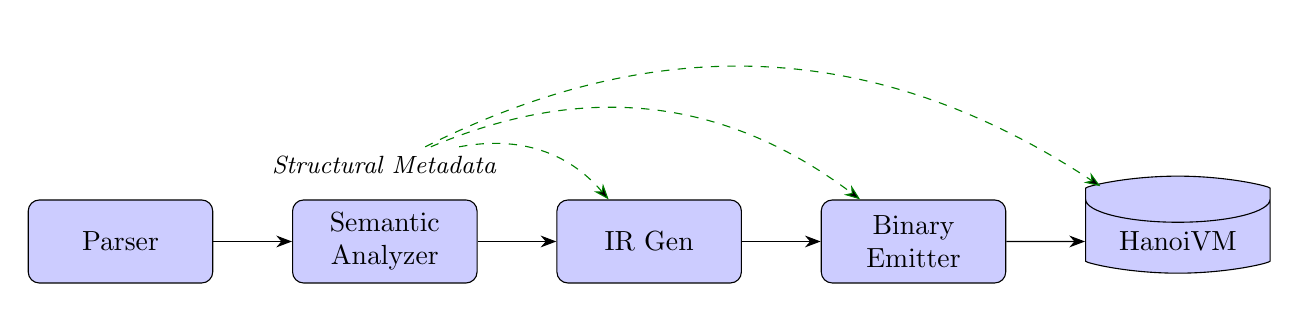
\begin{tikzpicture}[
    node distance=1.5cm and 1cm,
    block/.style={rectangle, draw, fill=blue!20, text width=6em, text centered, rounded corners, minimum height=3em},
    meta/.style={draw=green!50!black, dashed, -{Stealth[length=2mm]}},
    flow/.style={draw=black, solid, -{Stealth[length=2mm]}}
]
\node[block] (parser) {Parser};
\node[block, right=of parser] (analyzer) {Semantic Analyzer};
\node[block, right=of analyzer] (ir) {IR Gen};
\node[block, right=of ir] (binary) {Binary Emitter};
\node[block, shape=cylinder, right=of binary, shape border rotate=90, aspect=0.25] (vm) {HanoiVM};
\draw[flow] (parser) -- (analyzer);
\draw[flow] (analyzer) -- (ir);
\draw[flow] (ir) -- (binary);
\draw[flow] (binary) -- (vm);
\node[above=0.2cm of analyzer] (meta_label) {\small \textit{Structural Metadata}};
\draw[meta] (meta_label) edge[bend left] (ir);
\draw[meta] (meta_label) edge[bend left] (binary);
\draw[meta] (meta_label) edge[bend left] (vm);
\end{tikzpicture}
\caption{The T81 compiler pipeline, illustrating the persistent flow of structural metadata from the semantic analyzer through to the HanoiVM runtime.}
\label{fig:pipeline}
\end{figure}
\subsection{End-to-End Determinism Results}
The most critical claim of our work is reproducibility of `.tisc` artifacts under controlled build conditions. Validation is implemented as an operational gate rather than a one-off claim: cross-arch reproducibility scripts and CI workflows compare deterministic outputs and fail on drift. Table \ref{tab:reproducibility} summarizes the reproducibility gate model used in the repository.
\begin{table}[h]
\centering
\caption{Reproducibility gate summary. Concrete artifact hashes are tracked in CI outputs and reproducibility ledgers rather than hard-coded in this manuscript.}
\label{tab:reproducibility}
\begin{tabular}{|l|l|l|}
\hline
\textbf{Gate} & \textbf{Scope} & \textbf{Status Model} \\
\hline
T81Lang repro gate & Compiler/IR determinism & Pass/fail in CI (`t81lang_repro_gate.py`) \\
T3\_K repro gate & Quantization determinism & Pass/fail in CI (`t3k_repro_gate.py`) \\
Repro ledger workflow & Scheduled evidence artifacts & Pass/fail + archived artifacts \\
Runtime contract sync & Cross-repo boundary pinning & Pass/fail (`check-runtime-contract-sync.py`) \\
\hline
\end{tabular}
\end{table}
\subsection{Performance of Real Workloads}
To be a viable platform, a deterministic stack must still offer acceptable performance. We evaluate our system on a set of micro and macro-benchmarks to characterize its performance, from native ternary arithmetic to full ML model execution. The results are summarized in Table \ref{tab:perf_summary}.
\begin{table}[h]
\centering
\caption{Performance Summary Across Workloads}
\label{tab:perf_summary}
\begin{tabular}{|l|c|c|}
\hline
\textbf{Workload} & \textbf{Metric} & \textbf{Result} \\
\hline
NegationSpeed (classic path) & Throughput & 24.96 Gops/s (benchmark snapshot) \\
NegationSpeed (native SIMD path) & Throughput & 40.93 Gops/s (benchmark snapshot) \\
Llama RMSNorm/SiLU/Softmax & Throughput ratio vs binary baseline & 31.63x / 7.27x / 7.05x \\
\hline
\end{tabular}
\end{table}
The benchmark profile is mixed by design stage and workload: several ternary-native kernels show strong gains, while wide integer arithmetic and selected file-system or conversion pathways remain behind binary baselines in the current snapshot. These results should therefore be interpreted as a moving systems profile, not a single scalar claim. They establish both where ternary-native execution is already competitive and where further kernel/JIT work is still required.
\begin{figure}[h]
\centering
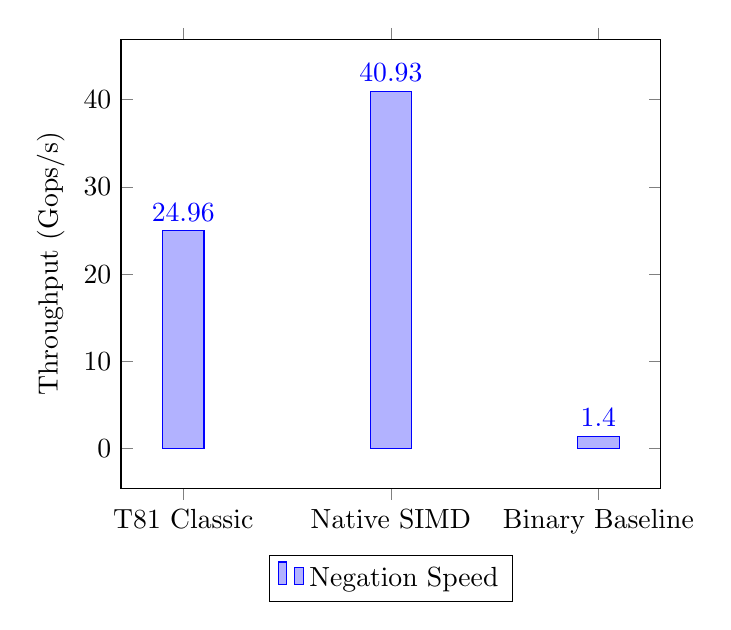
\begin{tikzpicture}
\begin{axis}[
    ybar,
    bar width=15pt,
    enlargelimits=0.15,
    legend style={at={(0.5,-0.15)},
      anchor=north,legend columns=-1},
    ylabel={Throughput (Gops/s)},
    symbolic x coords={T81 Classic, Native SIMD, Binary Baseline},
    xtick=data,
    nodes near coords,
    nodes near coords align={vertical},
    ]
\addplot coordinates {(T81 Classic,24.96) (Native SIMD,40.93) (Binary Baseline,1.40)};
\legend{Negation Speed}
\end{axis}
\end{tikzpicture}
\caption{Negation benchmark throughput comparison (from `docs/benchmarks.md`, 2026-02-09). Ternary paths outperform binary baseline.}
\label{fig:negation_bench}
\end{figure}
\begin{figure}[h]
\centering
\begin{lstlisting}
+--------------------------+---------------+----------+
| Benchmark | Time | Iterations|
+--------------------------+---------------+----------+
| BM_NegationSpeed (T81) | 24.96 Gops/s | (snapshot)|
| BM_NegationSpeed (Native)| 40.93 Gops/s | (snapshot)|
| BM_NegationSpeed (Binary)| 1.40 Gops/s | (snapshot)|
+--------------------------+---------------+----------+
\end{lstlisting}
\caption{Representative benchmark snapshot from the repository (`docs/benchmarks.md`, 2026-02-09).}
\label{fig:benchmark_screenshot}
\end{figure}
\subsection{Threats to Validity}
We acknowledge several limitations to our current work. The performance of the HanoiVM, while stable, is not yet competitive with highly optimized, JIT-compiled native code, as shown in our evaluation. The overhead of our metadata-driven approach and the interpreted nature of the VM are subjects of ongoing performance analysis. Our evaluation currently focuses on a single workload, and further research is needed to validate the performance characteristics on a broader range of applications. Finally, the HanoiVM is currently single-threaded, which limits its applicability for highly parallel tasks. We believe, however, that these are engineering challenges that can be addressed within our foundational deterministic framework, rather than fundamental flaws in the approach itself.
\section{Related Work}
Our work builds on ideas from reproducible builds, canonical serialization formats, and modern systems languages. We position our contribution relative to these areas.
\begin{table*}[t]
\centering
\caption{Comparison of Determinism Approaches}
\label{tab:related_work_table}
\begin{tabular}{|l|l|l|l|}
\hline
\textbf{System / Approach} & \textbf{Scope of Determinism} & \textbf{Mechanism} & \textbf{Key Limitation (from our perspective)} \\
\hline
Reproducible Builds (Nix, Bazel) & Native binary & Hermetic build environments, fixed toolchains & Loses structural metadata; environment is complex to manage \\
Canonical Serialization (Cap'n Proto) & Data interchange format & Fixed-width fields, no pointers, strict layout rules & Solves data determinism, not code or layout determinism \\
Rust / Zig & Native binary (goal) & Best-effort compiler flags, controlled toolchains & Still sensitive to linker/system variance; metadata is debug-only \\
MLIR & Multi-level IR & Dialects and progressive lowering & Optimization-focused, potential semantic drift in passes \\
TVM & Deep learning compiler & End-to-end graph optimization & Performance portability but version-dependent inference drift \\
\textbf{T81 Foundation} & \textbf{VM Binary + Runtime Layout} & \textbf{Language semantics + Metadata propagation} & \textbf{Introduces VM interpretation overhead} \\
\hline
\end{tabular}
\end{table*}
\textbf{Reproducible Builds.} The reproducible builds movement, embodied by projects like Nix/Guix \cite{nix} and build systems like Bazel \cite{bazel}, has made enormous progress in taming the non-determinism of native toolchains. These systems work by creating highly controlled, hermetic build environments where every dependency, from the C library to the compiler itself, is pinned to a specific version. This allows them to produce bit-identical native binaries, a practice successfully adopted by security-sensitive projects like Tor and Bitcoin Core. However, this approach has two drawbacks from the perspective of our threat model. First, it requires managing a complex and fragile build environment. Second, and more importantly, the resulting native binary is still a "semantic void"---all the high-level structural information from the source code has been erased. Our work complements these efforts by shifting the determinism guarantee from the build environment to the language and VM architecture itself.
\textbf{Canonical Serialization Formats.} Systems like Cap'n Proto \cite{capnproto} and FlatBuffers \cite{flatbuffers} provide schemas for defining data structures that have a single, canonical serialized representation. This is crucial for deterministic data interchange. These systems solve half the problem: they ensure data is read and written consistently. However, they do not address the determinism of the code that operates on that data, nor do they guarantee that the in-memory layout of the data will be deterministic. The T81 Foundation applies the core idea of canonical serialization not just to data, but to the entire program: its code, its data, and its metadata are all part of a single, canonical binary format.
\textbf{Modern Systems Languages.} Languages like Rust \cite{rust} and Zig \cite{zig} have made deterministic builds a design goal. However, because they target native binaries, they are fundamentally at the mercy of the underlying system's toolchain (e.g., the linker). While they provide options to mitigate non-determinism, achieving bit-identical results across different platforms remains a significant challenge. Crucially, in these languages, the rich type information that could be used to enforce deterministic layouts at runtime is treated as debug information and is not a core part of the program's execution model. Our key contribution is to make this metadata a first-class citizen, not just at compile time, but at runtime, and to use it as the primary mechanism for ensuring verifiable determinism.
\section{Conclusion and Future Work}
The T81 Foundation provides a model for building trustworthy computational systems by enforcing metadata preservation, canonicalization boundaries, and transparent tooling. Current results show that these guarantees are operationally testable via regression and reproducibility gates, while performance remains workload-dependent. Future work focuses on kernel optimization, broader reproducibility matrices, and JIT/runtime improvements while preserving deterministic semantics. We view this as a practical path toward auditable and replayable AI-relevant computation rather than a claim of universal performance parity. Join @t81dev on X for updates and contributions.
\section{Acknowledgments}
We thank the open-source community for their invaluable contributions and the anonymous reviewers for their constructive feedback.
\bibliographystyle{ACM-Reference-Format}
\begin{thebibliography}{12}
\bibitem{rust}
Klabnik, S. and Nichols, C. 2019. The Rust Programming Language (2nd ed.). No Starch Press.

\bibitem{zig}
Zig Software Foundation. 2024. The Zig Programming Language. \url{https://ziglang.org}.

\bibitem{swift}
Apple Inc. 2024. The Swift Programming Language. \url{https://docs.swift.org/swift-book/}.

\bibitem{mlir}
Lattner, C., Amini, M., Bondhugula, U., Cohen, A., Davis, A., Pienaar, J., Riddle, R., Shpeisman, T., Vasilache, N., and Zinenko, O. 2020. MLIR: A Compiler Infrastructure for the End of Moore's Law. \textit{arXiv preprint arXiv:2002.11054}.

\bibitem{tvm}
Chen, T., Moreau, T., Jiang, Z., Zheng, L., Yan, E., Shen, H., Cowan, M., Wang, L., Hu, Y., Ceze, L., Guestrin, C., and Krishnamurthy, A. 2018. TVM: An Automated End-to-End Optimizing Compiler for Deep Learning. \textit{13th USENIX Symposium on Operating Systems Design and Implementation (OSDI 18)}. USENIX Association, 578--594.

\bibitem{mojo}
Modular Inc. 2023. Mojo Programming Language. \url{https://www.modular.com/mojo}.

\bibitem{setun}
Brusentsov, N. P. and Alvarez, J. R. 2011. Ternary Computers: The Setun and the Setun 70. In \textit{Perspectives on Soviet and Russian Computing}. Springer, 74--80. DOI:https://doi.org/10.1007/978-3-642-22816-2_10.

\bibitem{nix}
Dolstra, E., de Jonge, M., and Visser, E. 2004. Nix: A Safe and Policy-Free System for Software Deployment. In \textit{Proceedings of the 18th USENIX Conference on System Administration (LISA '04)}. USENIX Association, 79--92.

\bibitem{bazel}
Google. 2024. Bazel: A Fast, Scalable, Multi-Language and Extensible Build System. \url{https://bazel.build}.

\bibitem{capnproto}
Varda, K. 2013. Cap'n Proto: Serialization/RPC System. \url{https://capnproto.org}.

\bibitem{flatbuffers}
Google. 2024. FlatBuffers: Memory Efficient Serialization Library. \url{https://flatbuffers.dev}.

\bibitem{ieee754}
IEEE Computer Society. 2019. IEEE Standard for Floating-Point Arithmetic. \textit{IEEE Std 754-2019 (Revision of IEEE 754-2008)}. IEEE. DOI:https://doi.org/10.1109/IEEESTD.2019.8766229.

\end{thebibliography}
\appendix
\section{HanoiVM Instruction Set}
The HanoiVM instruction set is designed for simplicity and close correspondence with the semantics of T81Lang. Table \ref{tab:hanoi_opcodes} lists a selection of representative opcodes.
\begin{table}[h]
\centering
\caption{Representative HanoiVM Opcodes}
\label{tab:hanoi_opcodes}
\begin{tabular}{|l|l|}
\hline
\textbf{Opcode} & \textbf{Description} \\
\hline
\texttt{NOP} & No operation. \\
\texttt{HALT} & Halt execution. \\
\texttt{LOAD\_CONST <idx>} & Load constant from pool at index. \\
\texttt{STORE\_VAR <idx>} & Store register to variable slot. \\
\texttt{LOAD\_VAR <idx>} & Load variable from slot to register. \\
\texttt{ADD, SUB, MUL, DIV} & Core arithmetic operations. \\
\texttt{MOD, NEG} & Remainder and negation. \\
\texttt{AND, OR, NOT} & Bitwise logical operations. \\
\texttt{EQ, NEQ, LT, GT, LTE, GTE} & Comparison operations. \\
\texttt{JUMP <addr>} & Unconditional jump. \\
\texttt{JUMP\_IF\_ZERO <addr>} & Jump if register is zero. \\
\texttt{JUMP\_IF\_NOT\_ZERO <addr>} & Jump if register is not zero. \\
\texttt{CALL <addr>} & Call a function. \\
\texttt{RETURN} & Return from a function. \\
\texttt{MAKE\_RECORD <type>} & Allocate a new record instance. \\
\texttt{GET\_FIELD <reg>, <fld>} & Get a field from a record. \\
\texttt{SET\_FIELD <reg>, <fld>} & Set a field in a record. \\
\texttt{MAKE\_OPTION\_SOME} & Wrap value in `Some`. \\
\texttt{MAKE\_OPTION\_NONE} & Create a `None` value. \\
\texttt{UNWRAP\_OPTION} & Unwraps a `Some`, may trap on `None`. \\
\texttt{OPTION\_IS\_SOME} & Check if an `Option` is `Some`. \\
\texttt{MAKE\_RESULT\_OK} & Wrap value in `Ok`. \\
\texttt{MAKE\_RESULT\_ERR} & Wrap value in `Err`. \\
\texttt{UNWRAP\_RESULT} & Unwraps an `Ok`, may trap on `Err`. \\
\texttt{RESULT\_IS\_OK} & Check if a `Result` is `Ok`. \\
\hline
\end{tabular}
\end{table}
\end{document}